\chapter{Feature Description}
%MAX 2 PAGES
Our program offers a variety in features. In this chapter these features are described.
\section{Import}
To specify the data used in the data model we use an XML file. Using a file to specify the data makes our program generic and easy to use since the same XML file can be used more than one time.

In the XML file all the needed information of a file is found. The path to the file is specified as well as the delimiter used. For each column a data type is specified. 
\subsection{XML wizard}
\begin{figure}[h!]
\centering
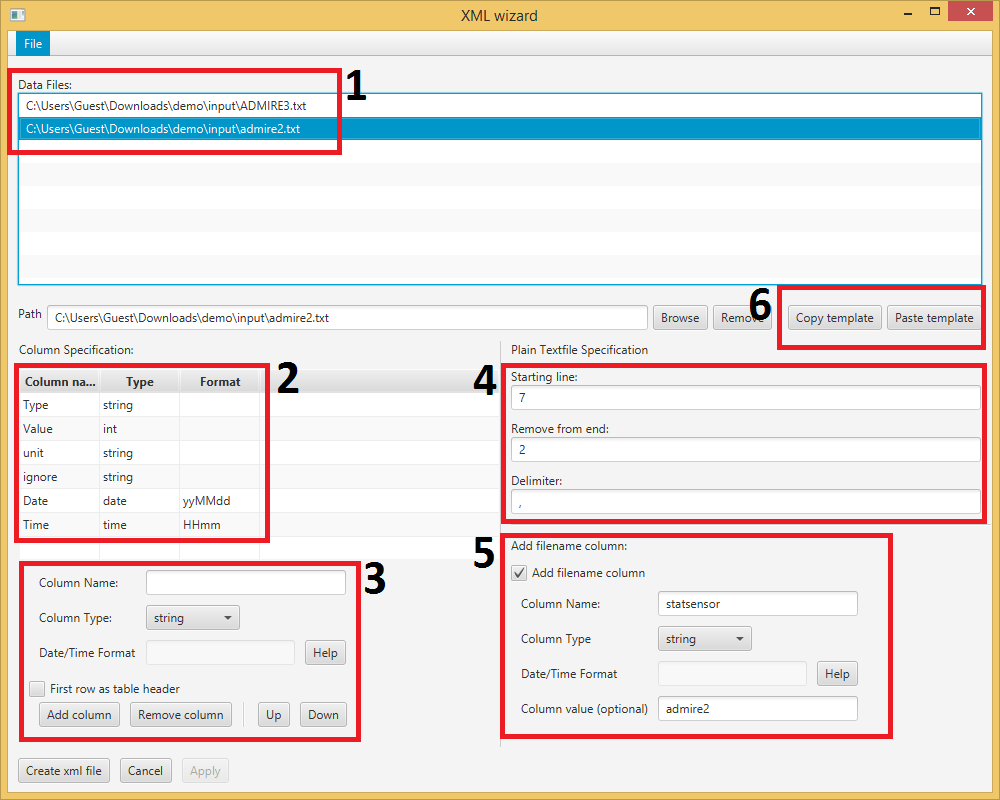
\includegraphics[width=300px]{chapters/image-featureDescription/xmlwizard-highlight.png}
\caption{The XML Wizard}
\end{figure}
To make it easier to make an XML file for our program, we created an XML wizard. In this wizard multiple files can be selected for the data [1]. Then per file, columns can be added with the appropriate type and (if needed) format [2, 3]. An option exists to use the first row as the column names. When this option is selected, no name needs to be specified for the columns in the wizard. The lines to skip at the start and the end of the file can be specified [4] and an option is available to add an extra column to the data containing the file-name or text specified by the user [5]. When all the settings are set, this info can be copied and then pasted for a similar file [6]. As in the example, multiple StatSensor files are loaded and use the same settings. 
\section{Analysis}
To analyse the data, the user has to switch to the 'analysis' tab. In this tab a text area is present where the user can add code in the program exclusive "SUGAR" language. When a script already exists, this file can simply be loaded into the program. This script can be changed and executed to affect the data. After changes are made, the script can be saved to file again. 
\subsection{The C's}
Multiple different analyses exist to execute on data. Following the terminology of EDA we implemented 6 out of the Eight C's of the generic ESDA process \cite{analysis}:
\subsubsection{Constraint}
A constraint can be used to select specific values from a column. Numbers can be compared to constants or other columns. Constraints can also be combined with AND, OR and NOT operations. On date values, the extra constraints "before" and "after" are available. 
\subsubsection{Computation}
Number values can be added, divided, multiplied and subtracted. The modulo operation is available, as well as the square root and the power function. Date values can be added or subtracted and the relative difference can be computed. Separate date and time can be combined to one DateTime value, also the opposite; DateTime values can be split up to either date or time value. All the computations can also be used in the constraints in combination with column values or constants.
\subsubsection{Comparison}
To determine a relation between events, the lag sequential comparison is available. The lag sequential analysis will return a table chronologically sorted on the events.
%lag sequential
\subsubsection{Code}
Codes can be added to rows when a value of that row satisfies a constraint. A single row can contain zero or more codes. When a row contains a code, it can be selected via a specific constraint that selects only that code. 
\subsubsection{Chunking}
Chunks can be created with the group by function. A group by function can be applied on a column or on a constraint combined with a column. This creates a new table with the first column the value of the group, the following columns are created after the functions given by the user, applied to that column.
\subsubsection{Connections}
To connect two or more tables, a join function is available. Tables can be joined in multiple ways. The full join is available as well as a left, right and simple join.
\subsection{Additional Analyses}
Apart from the implemented C's, more functions can be used in the program.  
\subsubsection{Union}
Two tables can be unified with the union command. This creates a new table with only the rows that have the same values in both tables. Codes of the rows of the two tables are not taken into account when comparing, but when two rows are the same the codes of both rows are combined in the new table.
\subsubsection{Difference}
The opposite of the union is also possible, the difference operation. Two tables are subtracted and only unique rows are added to the resulting table.
\section{Visualize}
No analysis is finished without visualizing the data. A visualization shows the data in an easy and fast interpretable way. In the visualization tab of the program buttons can be pressed to show a pop-up where the data for that visualization can be specified. After a visualization is made, the image can be saved as PNG file.
\subsection{Box-plot}
A single box-plot can be created of one column with the FloatValue or IntValue type. This happens in the graph pop-up where first a table is selected and then the column can be selected. The support of creating multiple box-plots at once is not implemented but it is possible to save box-plots one by one.
\subsection{Bar-chart}
A bar-chart can also be made via the graph pop-up. For the bar chart's axes, two columns must be selected. An example for the x-axis could be the names of created chunks since these are unique. For the y-axis a column with NumberValues must be picked. 
\subsection{State-Transition-Matrix}
The state-transition-matrix has its own pop-up menu. When no codes are present, the pop-up shows an error message and no matrix can be created because codes represent the states in the matrix. When a table is selected, a column can be selected to define the order of the table. Then the user can select the codes to add in the state-transition-matrix. When the create button is pressed, a matrix is created with the amount of transitions between the selected states as values.
